\newpage
\subsection{Caso d'uso UC6: Ricerca API}
\label{UC6}
\begin{figure}[ht]
	\centering
	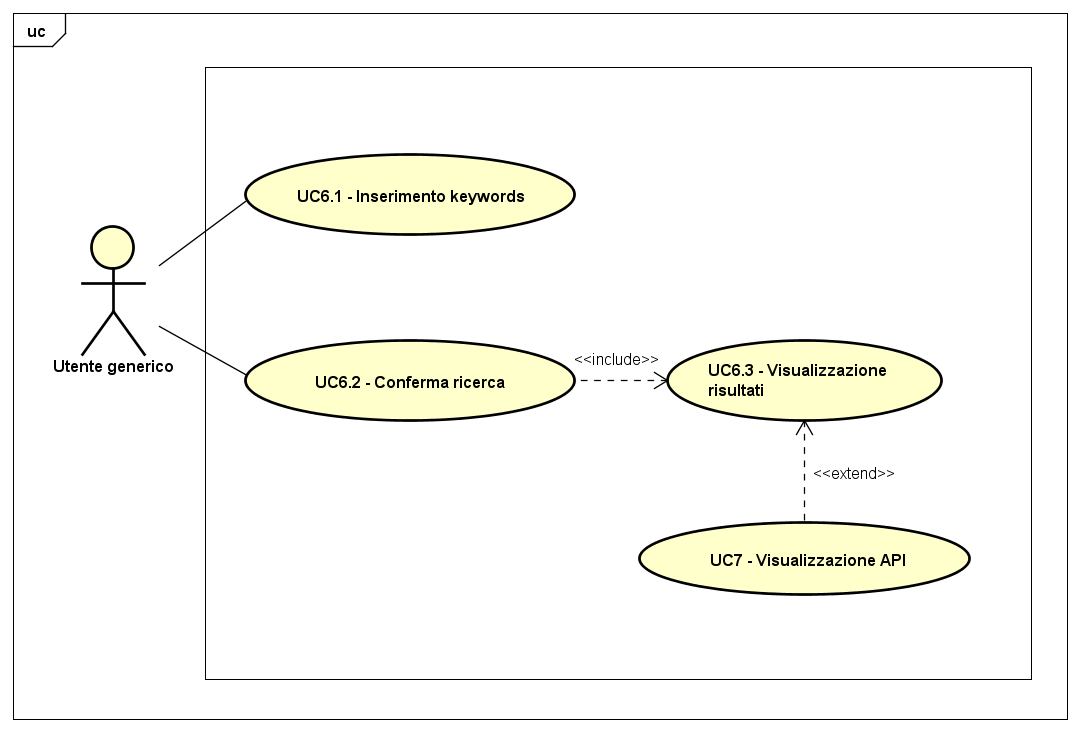
\includegraphics[scale=0.45]{UML/UC6.png}
	\caption{UC6: Ricerca API}
\end{figure}

\begin{longtable}{ l | p{11cm}}
	\hline
	\rowcolor{Gray}
	 \multicolumn{2}{c}{UC6 - Ricerca API} \\
	 \hline
	\textbf{Attori} & Utente generico, Utente non autenticato, Utente autenticato, Amministratore API Market \\
	\textbf{Descrizione} & L'attore inserisce le keywords per la ricerca di API \\
	\textbf{Pre-Condizioni} & L'attore ha scelto di effettuare una ricerca di API \\
	\textbf{Post-Condizioni} & L'attore ha effettuato la ricerca di API ed ha visualizzato la lista dei risultati \\
	\textbf{Scenario Principale} & 
	\begin{enumerate*}[label=(\arabic*.),itemjoin={\newline}]
		\item L'attore può inserire la stringa di ricerca desiderata (UC6.1)
		\item L'attore può confermare i dati inseriti (UC6.2) e visualizzare i risultati forniti dall'applicazione web (UC6.3)
	\end{enumerate*}\\
\end{longtable}

\subsubsection{Caso d'uso UC6.1: Inserimento keywords}
\label{UC6_1}

\begin{minipage}{\linewidth}
\begin{tabular}{ l | p{11cm}}
	\hline
	\rowcolor{Gray}
	 \multicolumn{2}{c}{UC6.1 - Inserimento keywords} \\
	 \hline
	\textbf{Attori} & Utente generico, Utente non autenticato, Utente autenticato, Amministratore API Market \\
	\textbf{Descrizione} & L'attore effettua una ricerca delle API inserendo nella barra di ricerca una stringa contenente le keywords desiderate \\
	\textbf{Pre-Condizioni} & L'attore ha scelto di effettuare una ricerca di API \\
	\textbf{Post-Condizioni} & L'attore ha inserito nella barra di ricerca una stringa contenente le keywords desiderate \\
	\textbf{Scenario Principale} & 
	\begin{enumerate*}[label=(\arabic*.),itemjoin={\newline}]
		\item L'attore può inserire nella barra di ricerca una stringa con tenente le keywords desiderate: esse verranno ricercate sul nome dell'API, sul nome dell'autore e su eventuali tag
	\end{enumerate*}\\
\end{tabular}
\end{minipage}

\subsubsection{Caso d'uso UC6.2: Conferma ricerca}
\label{UC6_2}

\begin{minipage}{\linewidth}
	\begin{tabular}{ l | p{11cm}}
		\hline
		\rowcolor{Gray}
		\multicolumn{2}{c}{UC6.2 - Conferma ricerca} \\
		\hline
		\textbf{Attori} & Utente generico, Utente non autenticato, Utente autenticato, Amministratore API Market \\
		\textbf{Descrizione} & L'attore conferma la stringa di ricerca inserita per poter visualizzare i risultati \\
		\textbf{Pre-Condizioni} & L'attore ha inserito una stringa di ricerca \\
		\textbf{Post-Condizioni} & L'attore ha confermato una stringa di ricerca \\
		\textbf{Scenario Principale} & 
		\begin{enumerate*}[label=(\arabic*.),itemjoin={\newline}]
			\item L'attore può confermare una stringa di ricerca, visualizzando la lista dei risultati (UC6.3)
		\end{enumerate*}\\
	\end{tabular}
\end{minipage}

\subsubsection{Caso d'uso UC6.3: Visualizzazione risultati}
\label{UC6_3}

\begin{minipage}{\linewidth}
	\begin{tabular}{ l | p{11cm}}
		\hline
		\rowcolor{Gray}
		\multicolumn{2}{c}{UC6.3 - Visualizzazione risultati} \\
		\hline
		\textbf{Attori} & Utente generico, Utente non autenticato, Utente autenticato, Amministratore API Market \\
		\textbf{Descrizione} & L'attore visualizza le API che corrispondono alle keywords della ricerca effettuata \\
		\textbf{Pre-Condizioni} & L'attore ha confermato la ricerca API \\
		\textbf{Post-Condizioni} & L'attore ha visualizzato le API che corrispondono alle keywords della ricerca effettuata \\
		\textbf{Scenario Principale} & 
		\begin{enumerate*}[label=(\arabic*.),itemjoin={\newline}]
			\item L'attore può visualizzare le API che corrispondono alle keywords della ricerca effettuata, che possono essere anche vuoti nel caso di stringhe non consone
		\end{enumerate*}\\
		\textbf{Scenari Alternativi} & 
		\begin{enumerate*}[label=(\arabic*.),itemjoin={\newline}]
		\item L'attore può accedere alla schermata delle singole API tramite la lista delle API (UC7)
	\end{enumerate*}\\
	\end{tabular}
\end{minipage}